\section{Linkage validation}
\label{app:linkage}

\subsection*{The regional reference}

A stratified review of 120 awarded digital anchors across Bretagne, Pays de la Loire and Normandie, carried
out on 11 August 2026 against the real BOAMP notices and their official URLs, before the linkage methods in
this project existed. 112 anchors re-resolve onto exactly one episode; 88 are usable. The pilot split holds
16 usable anchors (5 positive) and the locked split 72 (18 positive), with 5,221 and 20,917 candidate pair
rows respectively. The split is recorded in the reference file itself and is not post hoc.

Four limits bound its reach: the labels come from a single large-language-model research pass, spot-checked
rather than verified anchor by anchor; the per-anchor evidence trail was not recorded; negatives are
corpus-relative, because roughly 25 candidates per anchor were considered rather than the full pool; and the
rule that selected those 25 candidates was not recorded, so recall and the 0.913 candidate ceiling are not
fully independent of the score they bound. Precision is unaffected by the fourth limit.

\subsection*{Existence detection versus exact successor identity}

Two accountings answer different questions. Anchor-level accounting asks whether the system detected that a
successor exists. Exact-successor accounting asks whether it named the right one, so a wrong successor on a
positive anchor counts as one false positive \emph{and} one false negative. The project's headline figures
are the latter.

Method keys, as in the body: \texttt{M\_A} deterministic, \texttt{M\_B} text ranking (primary), \texttt{M\_C} weighted gated, \texttt{M\_D} Fellegi--Sunter.

\begin{longtable}[]{@{}lrrrrr@{}}
\toprule\noalign{}
Method (locked split) & Threshold & TP & FP & FN & TN \\
\midrule\noalign{}
\endhead
\multicolumn{6}{@{}l}{\emph{Existence detection (anchor level)}}\\
\texttt{M\_A} & n/a & 8 & 7 & 10 & 47 \\
\texttt{M\_B} & 0.70 & 8 & 0 & 10 & 54 \\
\texttt{M\_C} & 0.70 & 13 & 10 & 5 & 44 \\
\texttt{M\_D} & 0.65 & 4 & 1 & 14 & 53 \\
\midrule
\multicolumn{6}{@{}l}{\emph{Exact successor identity}}\\
\texttt{M\_A} & n/a & 8 & 7 & 10 & 47 \\
\texttt{M\_B} & 0.70 & 7 & 1 & 11 & 54 \\
\texttt{M\_C} & 0.70 & 12 & 11 & 6 & 44 \\
\texttt{M\_D} & 0.65 & 1 & 4 & 17 & 53 \\
\bottomrule\noalign{}
\end{longtable}

The gap between the two blocks is the whole point: \texttt{M\_C} detects five more anchors that do have a
successor, but names the wrong episode often enough that its exact-successor precision falls to 0.522.

\subsection*{Threshold sweep, \texttt{M\_B}, locked split}

\begin{longtable}[]{@{}rrrrrrr@{}}
\toprule\noalign{}
Threshold & Accepted & Correct & Precision & Recall & FPR & Coverage \\
\midrule\noalign{}
\endhead
0.50 & 21 & 10 & 0.476 & 0.556 & 0.167 & 0.292 \\
0.55 & 17 & 9 & 0.529 & 0.500 & 0.111 & 0.236 \\
0.60 & 13 & 9 & 0.692 & 0.500 & 0.056 & 0.181 \\
0.65 & 10 & 8 & 0.800 & 0.444 & 0.019 & 0.139 \\
\textbf{0.70} & \textbf{8} & \textbf{7} & \textbf{0.875} & \textbf{0.389} & \textbf{0.000} & \textbf{0.111} \\
0.75 & 7 & 6 & 0.857 & 0.333 & 0.000 & 0.097 \\
0.80 & 6 & 5 & 0.833 & 0.278 & 0.000 & 0.083 \\
\bottomrule\noalign{}
\end{longtable}

The row at 0.70 is the retained operating point. Git history records that the policy drew on inspection of
this designated locked stratum before the final pipeline was frozen. The table is therefore internal
validation and sensitivity evidence, not a fully untouched holdout. The operating point has not been moved
since, and the lower thresholds remain sensitivity arms rather than post-hoc replacements.

\begin{figure}[htbp]
\centering
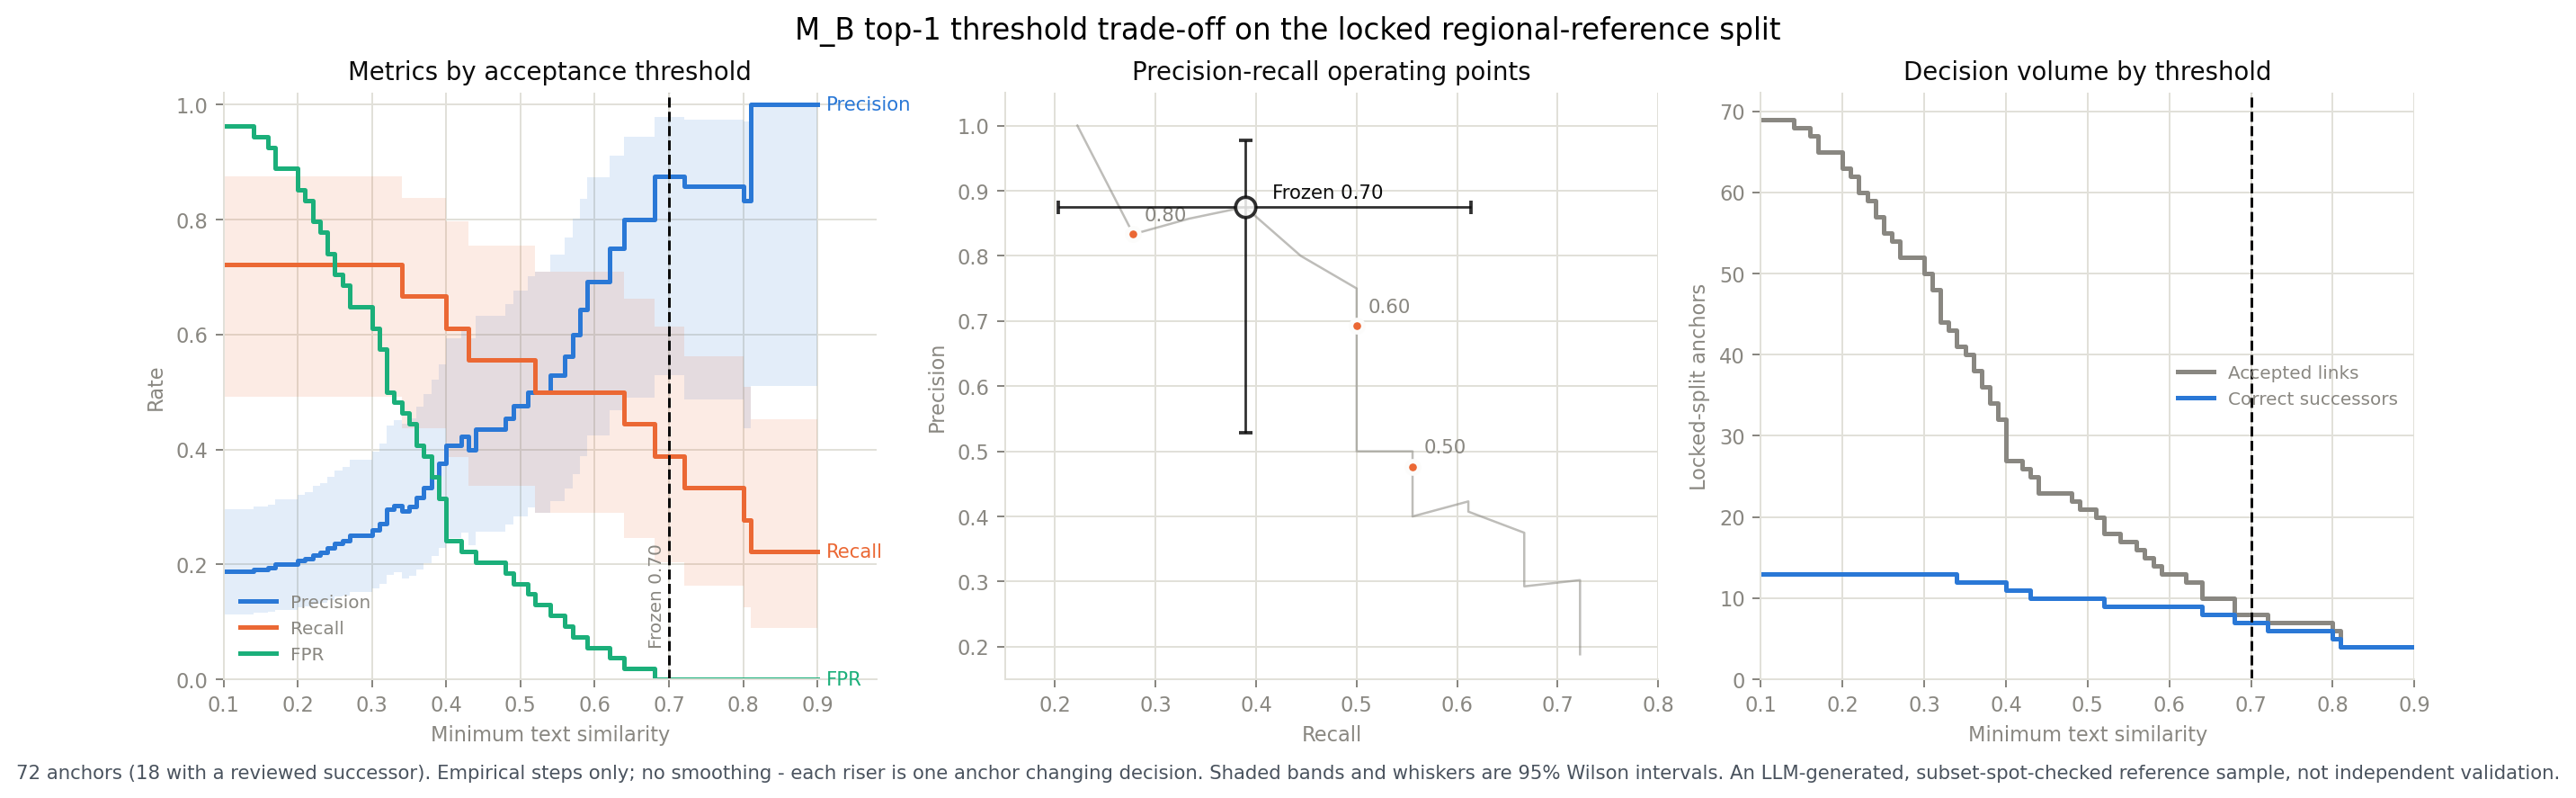
\includegraphics[width=\linewidth]{figures/fig05_threshold_tradeoff.png}
\caption{The complete threshold trade-off, all three panels. Left: precision, recall and false-positive rate against the acceptance threshold, with 95\,\% Wilson bands. Centre: the same information as precision--recall operating points, with the frozen 0.70 point and its interval marked. Right: how many anchors receive a link, and how many of those are the reviewed successor. The steps are empirical and unsmoothed: each riser is one anchor changing decision.}
\label{fig:appc-tradeoff}
\end{figure}

\subsection*{Pair-level ranking diagnostics}

\begin{longtable}[]{@{}lrrrr@{}}
\toprule\noalign{}
Method & ROC AUC & Average precision & Positive pairs & Negative pairs \\
\midrule\noalign{}
\endhead
\texttt{M\_A} & 0.7476 & 0.0378 & 16 & 20,901 \\
\texttt{M\_B} & 0.9915 & 0.4777 & 16 & 20,901 \\
\texttt{M\_C} & 0.9662 & 0.3452 & 16 & 20,901 \\
\texttt{M\_D} & 0.8383 & 0.0228 & 16 & 20,901 \\
\bottomrule\noalign{}
\end{longtable}

These curves rank scores; they do not measure accuracy at the acceptance threshold. The ROC AUC of 0.9915
does carry a real interpretation: on this internal reference, \texttt{M\_B} has a very high probability of
ranking a reviewed positive pair above a reviewed negative pair. With only 16 positive pairs among 20,917,
however, ROC AUC is less informative about the reliability of accepted positive links than precision--recall,
average precision and the anchor-level operating point \citep{davis2006,saito2015}. A second caveat applies to both: the 20,917 pairs come
from 69 anchors, so the observations are not independent and no clustered adjustment is made. The operating
point in the table above, not these curves, is what the event definition rests on.

\begin{figure}[htbp]
\centering
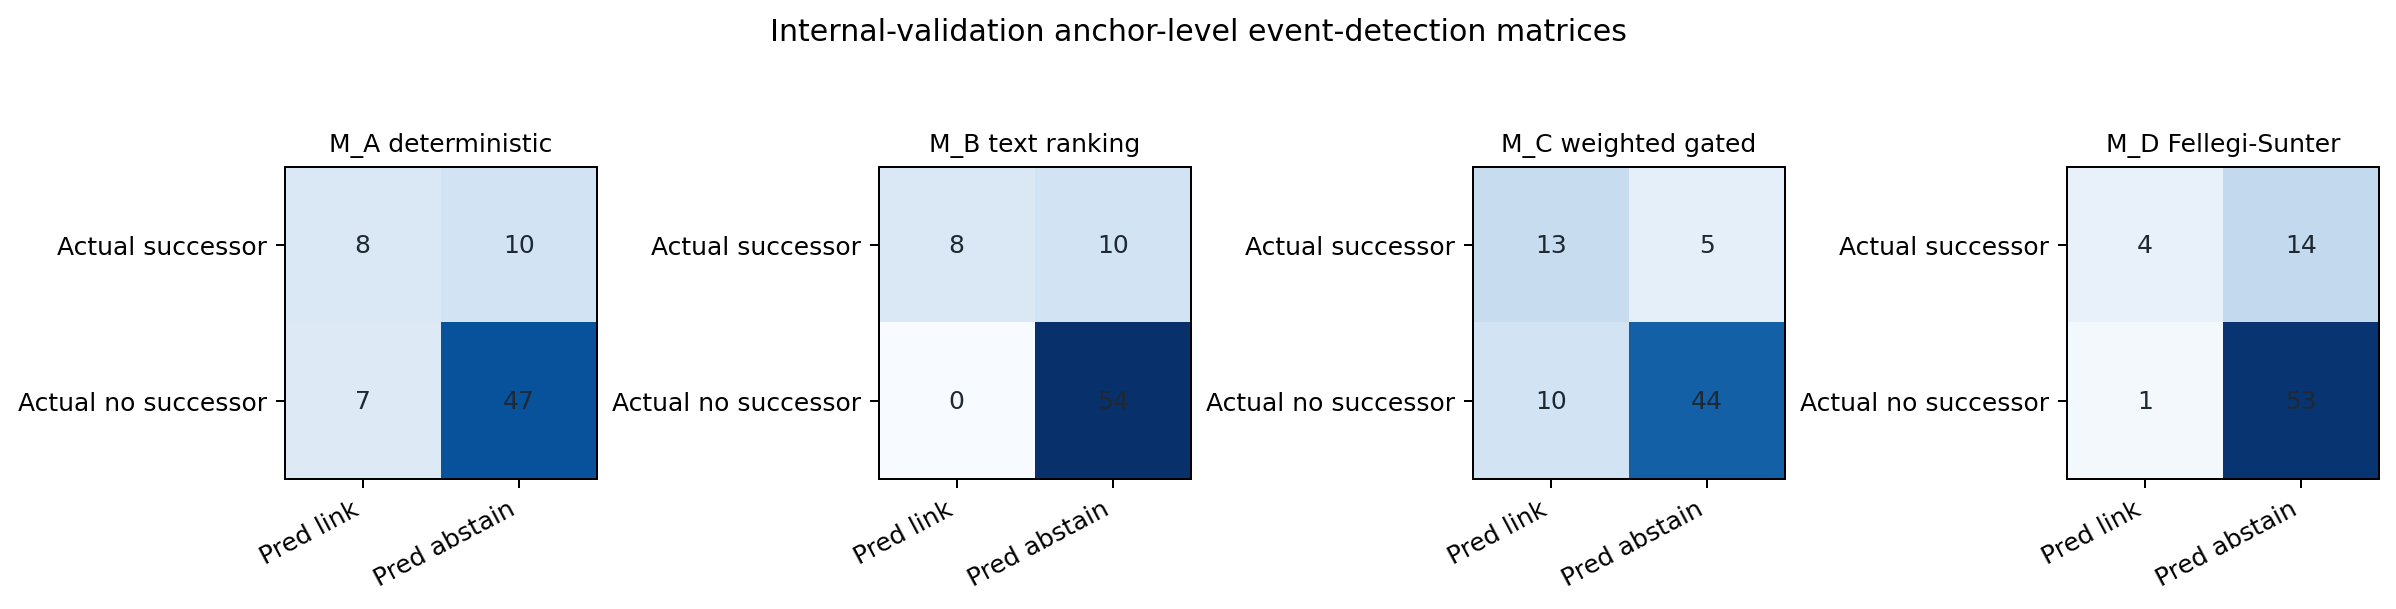
\includegraphics[width=0.9\linewidth]{figures/appC_confusion_matrices.png}
\caption{Anchor-level confusion matrices for the four linkage methods on the locked split. \texttt{M\_B} is
the only method with no accepted link on a reviewed-negative anchor; \texttt{M\_C} buys five additional
detections at the cost of ten.}
\label{fig:appc-cm}
\end{figure}

\begin{figure}[htbp]
\centering
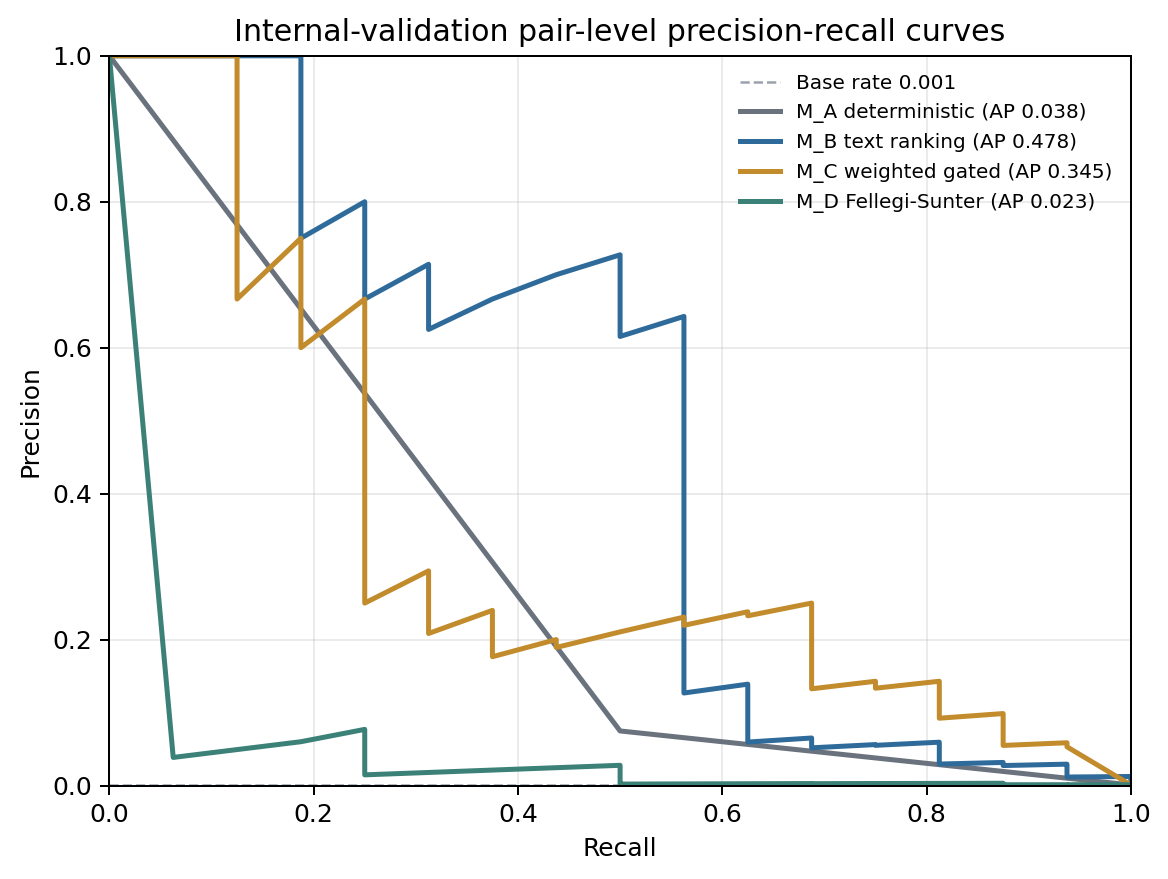
\includegraphics[width=0.72\linewidth]{figures/appC_pair_pr.png}
\caption{Pair-level precision--recall curves. The relevant diagnostic under extreme class imbalance, and the
one that shows how quickly precision degrades as recall is bought.}
\label{fig:appc-pr}
\end{figure}

\begin{figure}[htbp]
\centering
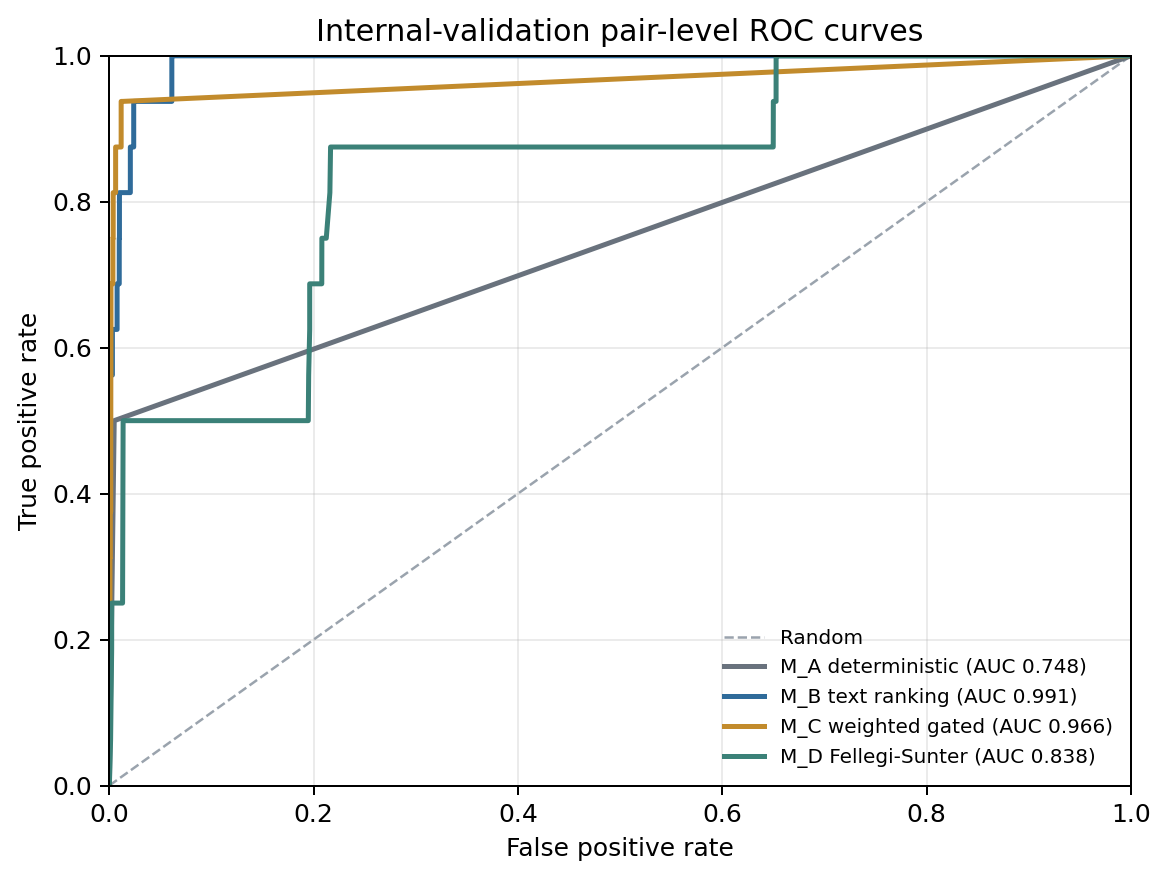
\includegraphics[width=0.72\linewidth]{figures/appC_pair_roc.png}
\caption{Pair-level ROC curves. \texttt{M\_B}'s AUC of 0.9915 indicates very strong pairwise ranking on the
internal reference. Under the 16-against-20,901 imbalance, precision--recall and anchor-level operating-point
metrics remain more decision-relevant for the reliability of accepted links.}
\label{fig:appc-roc}
\end{figure}

\subsection*{Candidate generation audit}

Candidate generation exposed 21 of the 23 reviewed successors, a pairs completeness of 0.913. Both
unreachable cases are attributed to a named blocking condition: one anchor never entered the cohort because
its award notice carries no structured Grand Ouest address, and one buyer changed legal form from CCAS to
CIAS with no shared SIREN. There are no unexplained cases, which is what separates an owned ceiling from an
implementation defect.

Of the 544 accepted links, 538 have a CPV division observed on both sides; 351 (65.2\,\%) stay within one
division. The reviewed reference successors cross divisions at a comparable rate, 9 of 23 (39.1\,\%), which
is why hard same-division blocking is not imposed: it would discard those 9 and cut the attainable recall
ceiling to 0.609. The buyer-blocking audit over the accepted links finds 0 conflicting validated SIRENs, 0
municipal / inter-municipal mixes, 18 name-only cross-department matches and 2 legal-family differences
flagged for review.

\subsection*{Challenge review}

A blinded 60-pair sample was prepared: 20 production-accepted links, 20 high-similarity structural negatives,
20 buyer-declared relationships, with a separate audit key and a pre-specified acceptance rule. The completed
review is model-assisted, not independent-human, and the repository records that provenance explicitly. Among
the 20 accepted links: 14 confirmed, 5 rejected, 1 uncertain, giving precision $14/19 = 0.737$ excluding the
uncertain row and $14/20 = 0.700$ on the conservative reading (exact 95\,\% interval $[0.457, 0.881]$). The
structural-negative stratum returned 19 negatives and 1 positive; the buyer-declared stratum 6 positives and
14 negatives, which demonstrates that a buyer-declared relationship is recruitment evidence rather than an
automatic successor label.
